\documentclass[12pt]{article}

\usepackage[a4paper, left=1.2in, right=1.2in]{geometry}
\usepackage{setspace}
\usepackage[utf8]{inputenc}
\usepackage[italian]{babel}
\usepackage[OT1]{fontenc}
\usepackage{graphicx}
\usepackage{subcaption}
\usepackage{float}
\usepackage{fancyhdr}
\usepackage{xcolor}
\usepackage{mathtools}
\usepackage{amsmath}
\usepackage{amssymb}
\usepackage{tikz}
\usepackage{imakeidx}
\usepackage{textcomp}
\usepackage{pifont}
\usepackage{polynom}
\usepackage{algorithm}
\usepackage{algpseudocode}
\usepackage{mathtools}
\usepackage{cancel}
\usepackage{pgfplots}
\usepackage{caption}
\usepackage{tabularx}
\usepackage{comment}
\usepackage{float}
\usepackage{bm}
\usepackage{multirow}
\usepackage{listings}
\usepackage[colorlinks=true,linkcolor=black,anchorcolor=black,citecolor=black,filecolor=black,menucolor=black,runcolor=black,urlcolor=black,backref=page]{hyperref}




\begin{document}


\lstset{ 
  language=Python,
  framesep=1pt,
  xleftmargin=0pt,
  framexleftmargin=0pt,
  frame=tb,
  framerule=1pt,
  breaklines=true,
  keywordstyle=\color{blue}\bfseries,
  showstringspaces=false
}
\begin{titlepage}
    \begin{center}
        
\includegraphics[scale=0.5]{images/uniba-logo.png}\\
        \vspace{0.5cm}
        % Dipartimento
        {\large COMPUTER SCIENCE DEPARTMENT}\\
        \vspace{0.5cm}
        % Corso di laurea
        {\large Computer Science - Curriculum Artificial Intelligence}\\
        \hrulefill \\
        \vspace{0.5cm}
        {\large Project Assignment}\\
        \vspace{0.5cm}
        % Materia
        {\large Formal Methods}\\
        \vspace{0.5cm}
        % Titolo
        {\LARGE \textbf{Process Mining}}
        \\ %% \textbf{Titolo della Tesi} 
        \vspace{0.5cm}

        \vfill
        \centering
        \begin{tabularx}{\textwidth}{@{}Xr@{}}
          % Relatore
          {\large Student:} &
          {\large \textit{Fontana Emanuele}} \\ 
        \end{tabularx}
        \textcolor{white}{.} \\ 
        \vspace{0.5cm}
        \hrulefill \\
        % Anno accademico in cui si è iscritti
        {\large Academic Year 2024/2025}
    \end{center}
\end{titlepage}
\newpage
\tableofcontents
\newpage
\section{Introduction to Process Mining}

\subsection{Petri Nets}

Petri nets are a mathematical and graphical model used to represent distributed and concurrent systems. In this model, systems are represented as networks composed of nodes and directed arcs. The nodes represent the states of the system, while the arcs represent transitions between these states. Petri nets are widely used in computer science to model complex systems, such as parallel processing systems, production control systems, and data processing systems.

\paragraph{Components of Petri Nets}
\begin{itemize}
    \item \textbf{Places}:
    \begin{itemize}
        \item Represent states or conditions within the system.
        \item Typically depicted as circles.
        \item A place can hold tokens that represent the system's current state.
    \end{itemize}
    \item \textbf{Transitions}:
    \begin{itemize}
        \item Represent events or actions that cause changes in the system.
        \item Typically depicted as rectangles or bars.
        \item A transition occurs (fires) when there are sufficient tokens in the connected places to satisfy the preconditions.
    \end{itemize}
    \item \textbf{Tokens}:
    \begin{itemize}
        \item Represent the dynamic state of the system at any given time.
        \item Tokens are placed in the places and can move through the network as transitions fire.
    \end{itemize}
\end{itemize}


\subsection{Process Mining}
Process mining is a discipline that uses data analysis techniques to improve the understanding and optimization of business processes. It relies on the digital recording of data related to business processes, which is then analyzed to identify opportunities for improvement and optimization. Process mining includes several techniques, such as process visualization, analysis of wait times and durations, automatic discovery of process models, and analysis of deviations from established models. The end result is a deeper understanding of business processes, which can be used to implement solutions for their optimization. Process mining is a valuable technology for many companies and organizations, as it helps identify inefficiencies in processes, reduce waiting times, and improve service quality to customers. Furthermore, process mining offers an intuitive visualization of business processes, which facilitates communication and collaboration among different stakeholders.

A process consists of actions (possibly concurrent) performed by agents (human or artifacts). Its dynamic behavior can be characterized in terms of events referring to identifiable actions (including decisions on the next task to be performed). Atomic activities are represented as single events, while activities that span a significant amount of time are represented by the interval between the start and end of the corresponding events. 

\subsubsection{Directly-Follows Graph (DFG)}

The \textbf{Directly-Follows Graph (DFG)} is a graphical representation used in \textit{process mining} to describe the direct relationships between activities in a process. In this graph:
\begin{itemize}
    \item The \textbf{nodes} represent the activities (or events) that occur in the process.
    \item The \textbf{edges} represent the direct "follows" relationship, meaning that one activity immediately follows another in the event log.
    \item The \textbf{direction of the edges} indicates the sequence of execution, with an edge from Activity A to Activity B meaning that Activity B directly follows Activity A.
    \item The \textbf{edge weight} often represents the frequency with which one activity follows another.
\end{itemize}

The DFG helps in visualizing the flow of the process and is often used as a foundation for process discovery algorithms, such as Alpha Miner, Inductive Miner, and Heuristic Miner.


\subsubsection{Alpha Miner}
The \textbf{Alpha Miner algorithm} is a foundational technique in \textit{process mining} used to discover process models from event logs. It reconstructs a workflow model, typically represented as a Petri net, based on the sequence and concurrency of events. Below is a brief explanation:

\paragraph{Key Concepts}
\begin{itemize}
    \item \textbf{Event Log}: A collection of traces, where each trace is a sequence of events (activities) performed during a process instance.
    \item \textbf{Causal Relations}: The algorithm identifies relationships between activities:
    \begin{itemize}
        \item \textit{Direct causality} ($A \rightarrow B$): Activity $A$ directly precedes activity $B$ in the log.
        \item \textit{Concurrency} ($A \parallel B$): Activities $A$ and $B$ can occur in any order, indicating parallel execution.
        \item \textit{No relation} ($A \# B$): No observable relationship between $A$ and $B$.
    \end{itemize}
\end{itemize}

\paragraph{Steps of the Alpha Miner Algorithm}
\begin{enumerate}
    \item \textbf{Preprocessing}: Parse the event log to extract traces and their activities.
    \item \textbf{Identify Relations}:
    \begin{itemize}
        \item Determine which activities are causally related, concurrent, or unrelated.
    \end{itemize}
    \item \textbf{Build a Petri Net}:
    \begin{itemize}
        \item Create \textit{places} (conditions) to represent causal dependencies.
        \item Add \textit{transitions} for each activity and connect them via places based on the identified relations.
    \end{itemize}
    \item \textbf{Generate Initial and Final Places}:
    \begin{itemize}
        \item Define the starting and ending conditions of the process.
    \end{itemize}
\end{enumerate}






\subsubsection{Inductive Miner Algorithm}

The \textbf{Inductive Miner algorithm} is a popular technique in \textit{process mining} that generates process models from event logs. Unlike the Alpha Miner, it guarantees the creation of sound workflow models by recursively dividing and conquering the event log data. Below is an overview of the algorithm:

\paragraph{Key Concepts}
\begin{itemize}
    \item \textbf{Event Log}: A collection of traces where each trace represents a sequence of activities in a process instance.
    \item \textbf{Behavioral Patterns}: The algorithm identifies the following key patterns in the event log:
    \begin{itemize}
        \item \textit{Sequence}: Activities follow each other in a strict order.
        \item \textit{Concurrency}: Activities can occur in parallel.
        \item \textit{Choice}: One activity is chosen from several alternatives.
        \item \textit{Loops}: Activities repeat a certain number of times.
    \end{itemize}
\end{itemize}

\paragraph{Steps of the Inductive Miner Algorithm}
\begin{enumerate}
    \item \textbf{Preprocessing}: Parse the event log and ensure it contains traces of activities with start and end points.
    \item \textbf{Partitioning the Log}:
    \begin{itemize}
        \item Divide the event log based on directly-follows relationships.
        \item Identify patterns (e.g., sequence, concurrency, choice, or loop) based on how activities relate to one another.
    \end{itemize}
    \item \textbf{Recursive Construction}:
    \begin{itemize}
        \item Create a submodel for each partition.
        \item Combine submodels using operators (\textit{sequence, concurrency, choice, loop}) to form the overall process model.
    \end{itemize}
    \item \textbf{Generate a Petri Net or Process Tree}:
    \begin{itemize}
        \item Translate the resulting model into a Petri net or process tree for visualization and analysis.
    \end{itemize}
\end{enumerate}


\subsubsection{Heuristic Miner Algorithm}

The \textbf{Heuristic Miner algorithm} is a process discovery technique used in \textit{process mining}. It extends the capabilities of the Alpha Miner by handling noise and incompleteness in event logs, making it more robust for real-world scenarios. The algorithm identifies causal relationships and constructs a dependency graph to represent the process.

\paragraph{Key Concepts}
\begin{itemize}
    \item \textbf{Event Log}: A collection of traces, where each trace is a sequence of events (activities) performed in a process instance.
    \item \textbf{Causal Dependency Measures}:
    \begin{itemize}
        \item \textit{Directly Follows Relation}: Determines if activity $A$ is frequently followed by activity $B$ in the log.
        \item \textit{Dependency Score}: Quantifies the strength of the causal relationship between activities based on their occurrence patterns.
    \end{itemize}
    \item \textbf{Thresholds}: Used to filter out weak or noisy relations, focusing only on the most significant dependencies.
    \item \textbf{Dependency Graph}: A directed graph where nodes represent activities, and edges indicate dependencies, weighted by their strength.
\end{itemize}

\paragraph{Steps of the Heuristic Miner Algorithm}
\begin{enumerate}
    \item \textbf{Preprocessing}: Parse the event log to extract traces and their activities.
    \item \textbf{Calculate Dependency Metrics}:
    \begin{itemize}
        \item Compute the frequency of directly follows relations between pairs of activities.
        \item Calculate the \textit{dependency score} for each pair to determine the strength of their causal relationship.
    \end{itemize}
    \item \textbf{Filter Relations}:
    \begin{itemize}
        \item Use predefined thresholds to remove weak or noisy relationships.
        \item Retain only significant dependencies.
    \end{itemize}
    \item \textbf{Construct a Dependency Graph}:
    \begin{itemize}
        \item Create a directed graph with nodes as activities and weighted edges as dependency scores.
    \end{itemize}
    \item \textbf{Generate a Process Model}:
    \begin{itemize}
        \item Convert the dependency graph into a workflow model, such as a Petri net or a process tree.
    \end{itemize}
\end{enumerate}

\subsubsection{Comparison}

\begin{table}[h!]
    \centering
    \renewcommand{\arraystretch}{1.3} % Adjust row height
    \begin{tabularx}{\textwidth}{|X|X|X|X|}
    \hline
    \textbf{Aspect}          & \textbf{Alpha Miner}                      & \textbf{Inductive Miner}              & \textbf{Heuristic Miner}               \\ \hline
    \textbf{Main Feature}    & Discovers simple process models           & Guarantees sound models               & Handles noise and incomplete event logs \\ \hline
    \textbf{Limitations}     & Sensitive to noise, struggles with complex loops & Limited to predefined patterns (e.g., sequence, loop) & Results depend on threshold settings   \\ \hline
    \end{tabularx}
    \caption{Comparison of Alpha Miner, Inductive Miner, and Heuristic Miner algorithms.}
    \label{tab:comparison}
    \end{table}

\subsubsection{Evaluation Metrics}


\begin{itemize}
    \item \textbf{Fitness}: It evaluates whether the model can reproduce the behavior observed in the log.
    
    \item \textbf{Precision}: It indicates whether the model allows execution sequences that were not present in the log.
    
    \item \textbf{Simplicity}: It evaluates the complexity of the discovered process model. A simpler model is typically more understandable and easier to analyze.
    
    \item \textbf{Generalization}: It measures the ability of the discovered model to handle unseen behavior beyond
\end{itemize}







\newpage
\section{Dataset}
\subsection{Introduction to the dataset}
Introduction to CASAS Dataset

In this study, we utilize a dataset from the Center for Advanced Studies in Adaptive Systems (CASAS). CASAS is a renowned research center focused on developing adaptive systems, particularly in the realm of smart environments and ubiquitous computing. The center provides a variety of datasets aimed at advancing the understanding and development of systems that interact intelligently with their surroundings.

The CASAS dataset contains data collected from sensor-equipped environments, typically used for applications such as activity recognition, healthcare monitoring, and smart home automation. These datasets often include information from sensors such as motion detectors, door sensors, temperature sensors, and other smart devices that track user behaviors and environmental conditions.

For process mining, CASAS datasets offer valuable insights into real-world human activities, allowing researchers to analyze patterns of behavior, optimize processes, and improve system performance. By using CASAS data, we can model and analyze the underlying processes, gaining a deeper understanding of complex behaviors in smart environments.

This dataset contains 1320 events and 3 attributes: Timestamp, CaseID, and Activity. The Timestamp attribute represents the date and time of each event, the CaseID attribute identifies the case to which the event belongs, and the Activity attribute describes the type of activity performed. The dataset is stored in a CSV file format, making it easy to process and analyze using various tools and techniques.

\subsection{Preprocessing}

Below is the Python code used for formatting a CSV file:

\begin{lstlisting}[caption={Format CSV Function}]
def format_csv(input_file, output_file):
    formatted_rows = []
    try:
        with open(input_file, 'r') as file:
            lines = file.readlines()
            formatted_rows.append("Timestamp, CaseID, Activity")
            for line in lines:
                line = line.strip()
                if not line:  # Ignore empty lines
                    continue
                elements = line.split()
                if len(elements) >= 4:  
                    timestamp = f"{elements[0]} {elements[1]}"
                    case_id = elements[2]
                    activity = ' '.join(elements[3:])
                    formatted_row = f"{timestamp}, {case_id}, {activity}"
                    formatted_rows.append(formatted_row)
        with open(output_file, 'w', newline='') as file:
            for row in formatted_rows:
                file.write(row + '\n')
    except Exception as e:
        print(f"A problem occurred while formatting the CSV file: {e}")
\end{lstlisting}

The function \texttt{format\_csv} reads a CSV file and formats it into a new CSV file with the columns \texttt{Timestamp}, \texttt{CaseID}, and \texttt{Activity}. The function extracts the timestamp, case ID, and activity from each line. It then writes the formatted rows to the output file.



\begin{lstlisting}[caption={CSV to XES Conversion}]
    def csv_to_xes(input_file):
        data = pd.read_csv(input_file, sep=",")
        cols = ['time:timestamp', 'case:concept:name','concept:name']
        data.columns = cols
        data['time:timestamp'] = pd.to_datetime(data['time:timestamp'])
        data['concept:name'] = data['concept:name'].astype(str)
        log = log_converter.apply(data, variant=log_converter.Variants.TO_EVENT_LOG)
        output_name = input_file.split(".")[0] + ".xes"
        write_xes.write_xes(log, output_name)
    \end{lstlisting}

The function \texttt{csv\_to\_xes} reads a CSV file and converts it into an XES file. It uses the \texttt{log\_converter} and \texttt{write\_xes} functions from the \texttt{pm4py} library to convert the CSV data into an event log. The event log is then written to an XES file with the same name as the input file.
\newpage
\section{Results}


\begin{figure}[H]
    \centering
    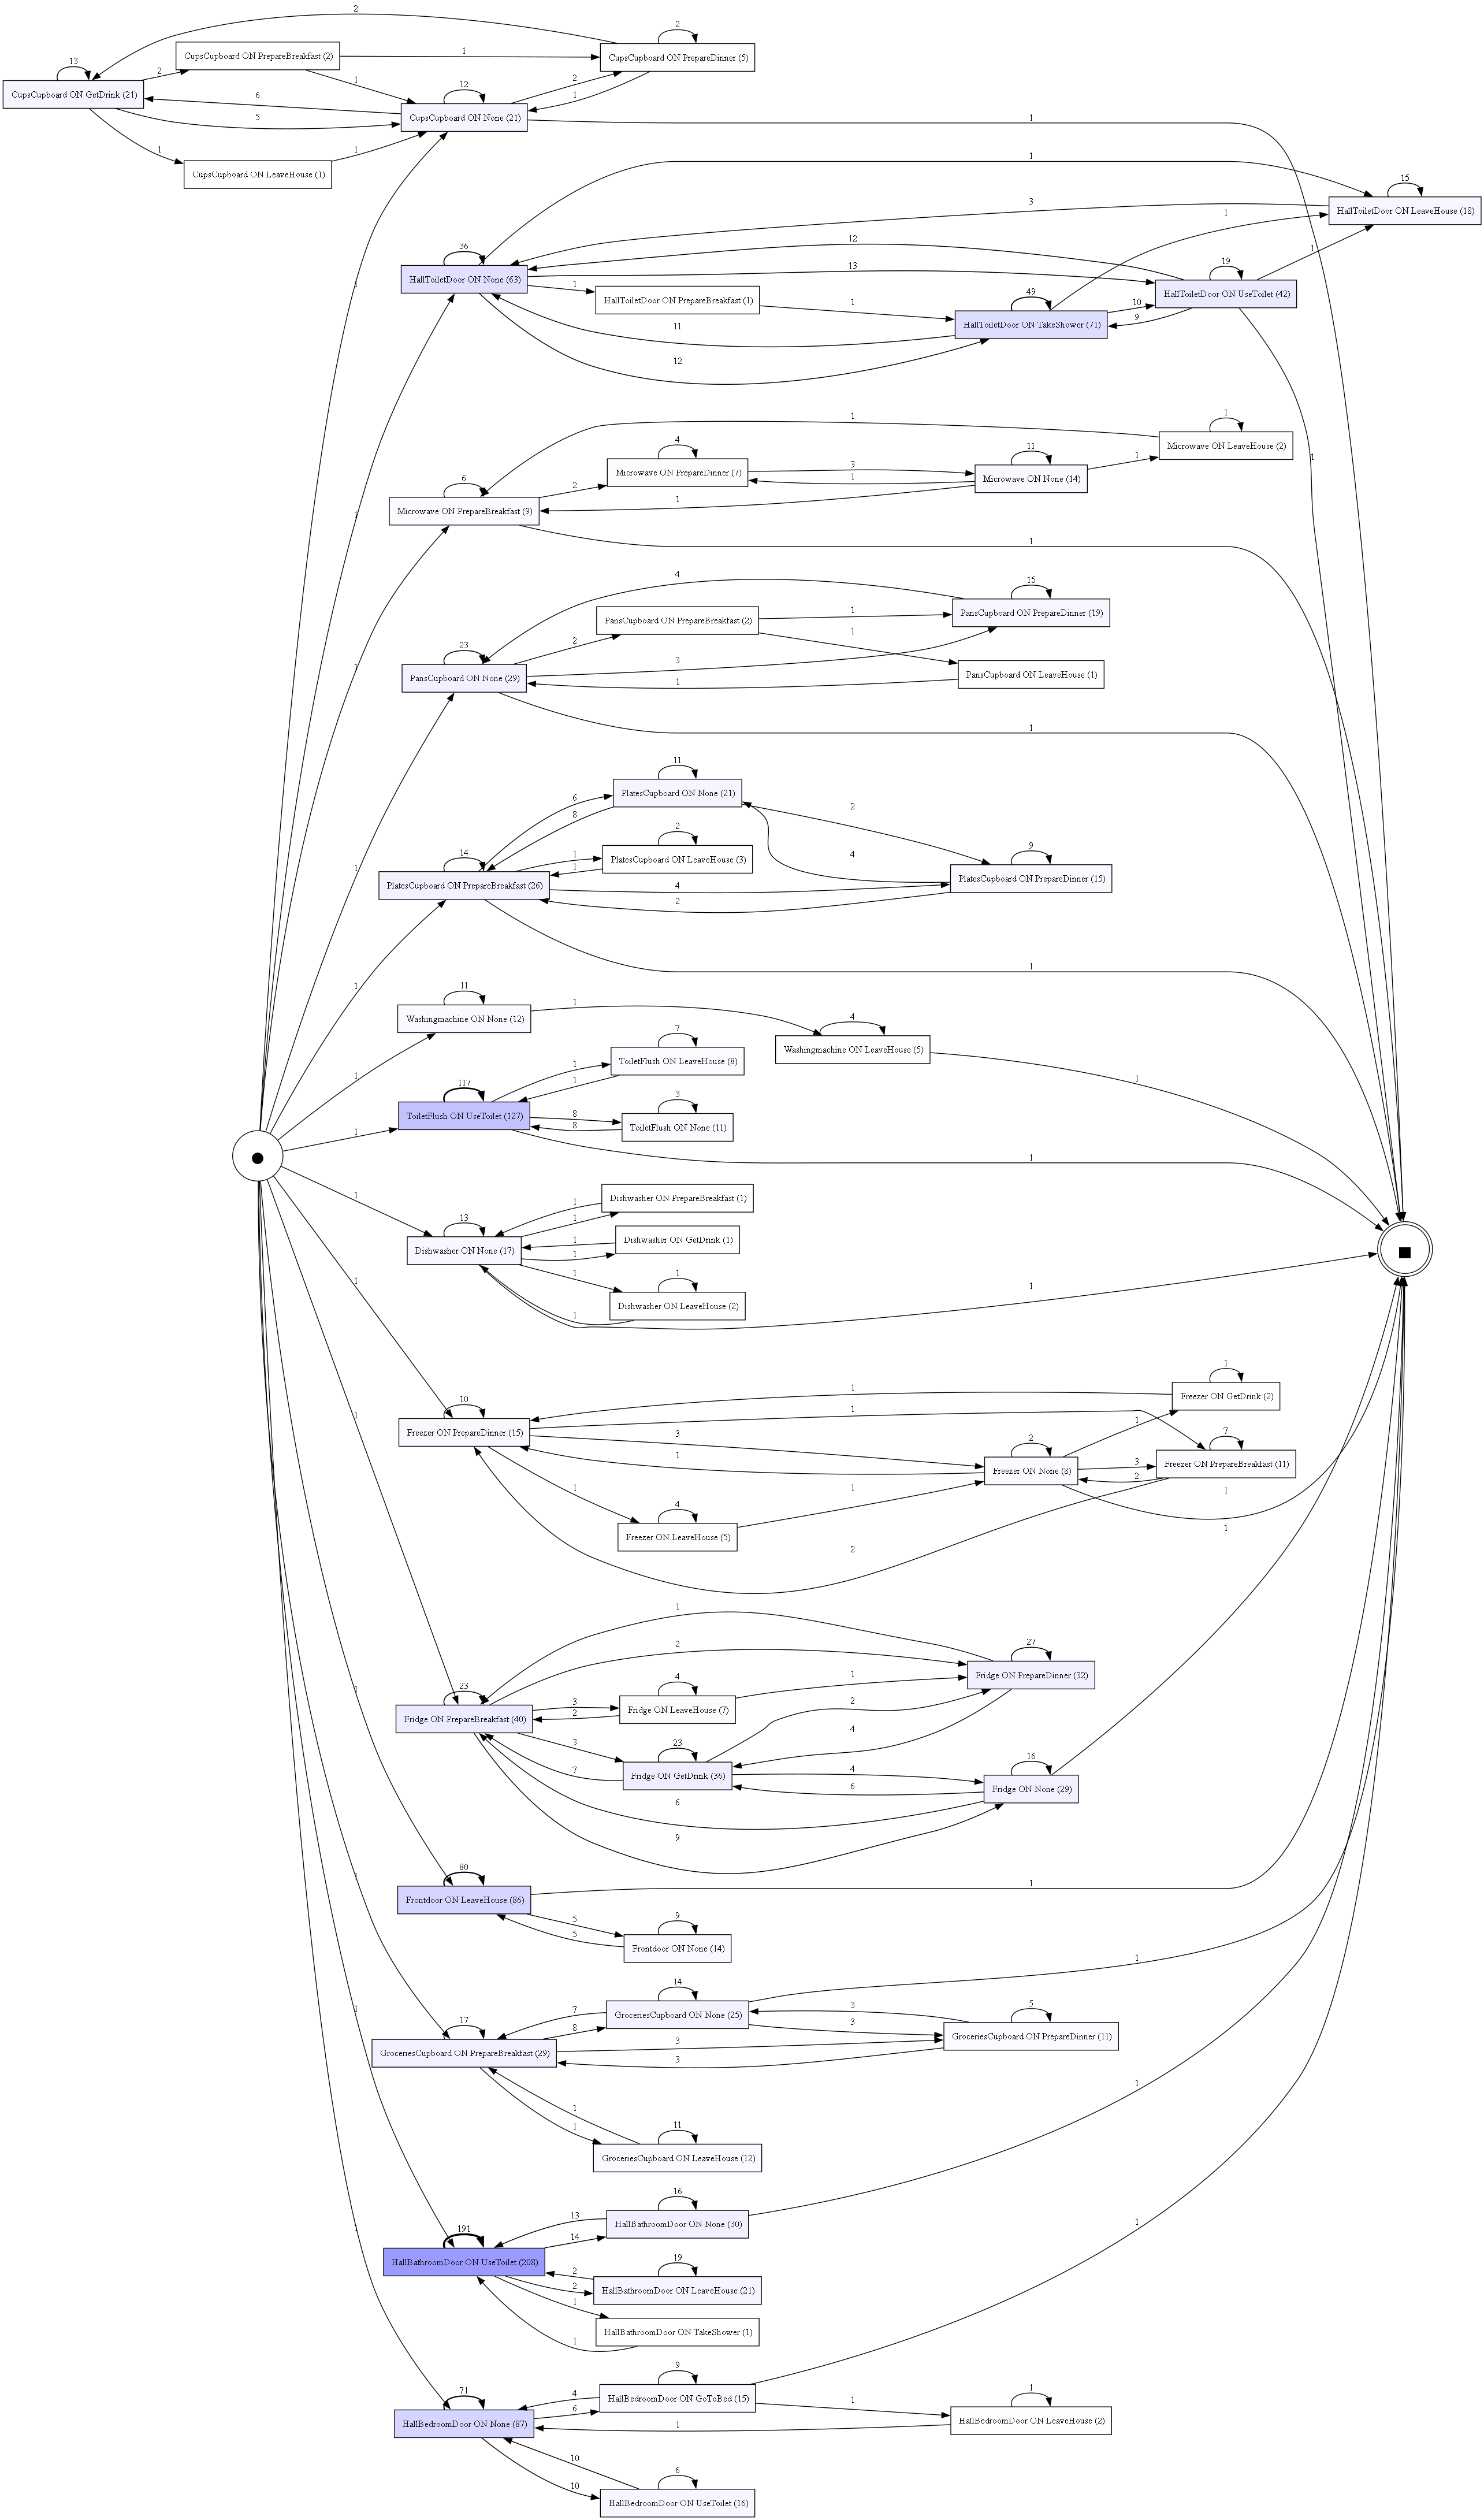
\includegraphics[width=\linewidth, height=\textheight]{images/dfg.png}
    \caption{Directly-Follows Graph (DFG) of the event log}
\end{figure}

\begin{figure}[H]
    \centering
    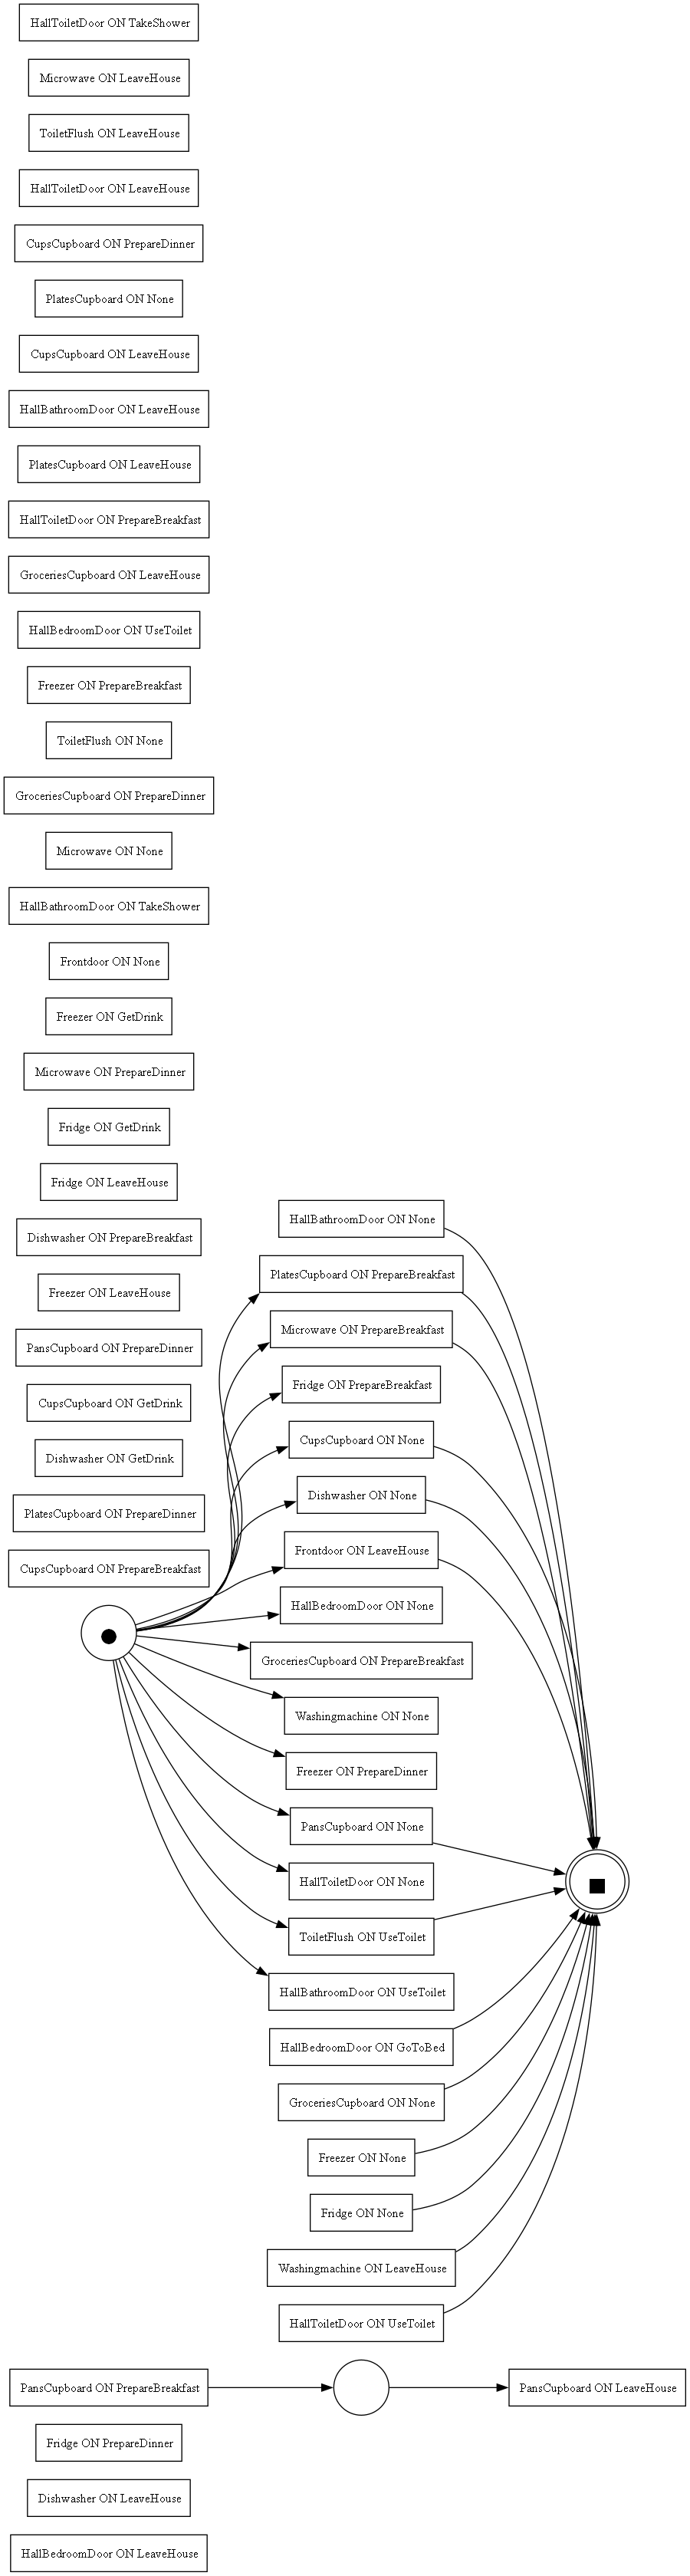
\includegraphics[width=\linewidth, height=\textheight]{images/alpha_miner.png}
    \caption{Alpha Miner Petri Net}
\end{figure}

\begin{figure}[H]
    \centering
    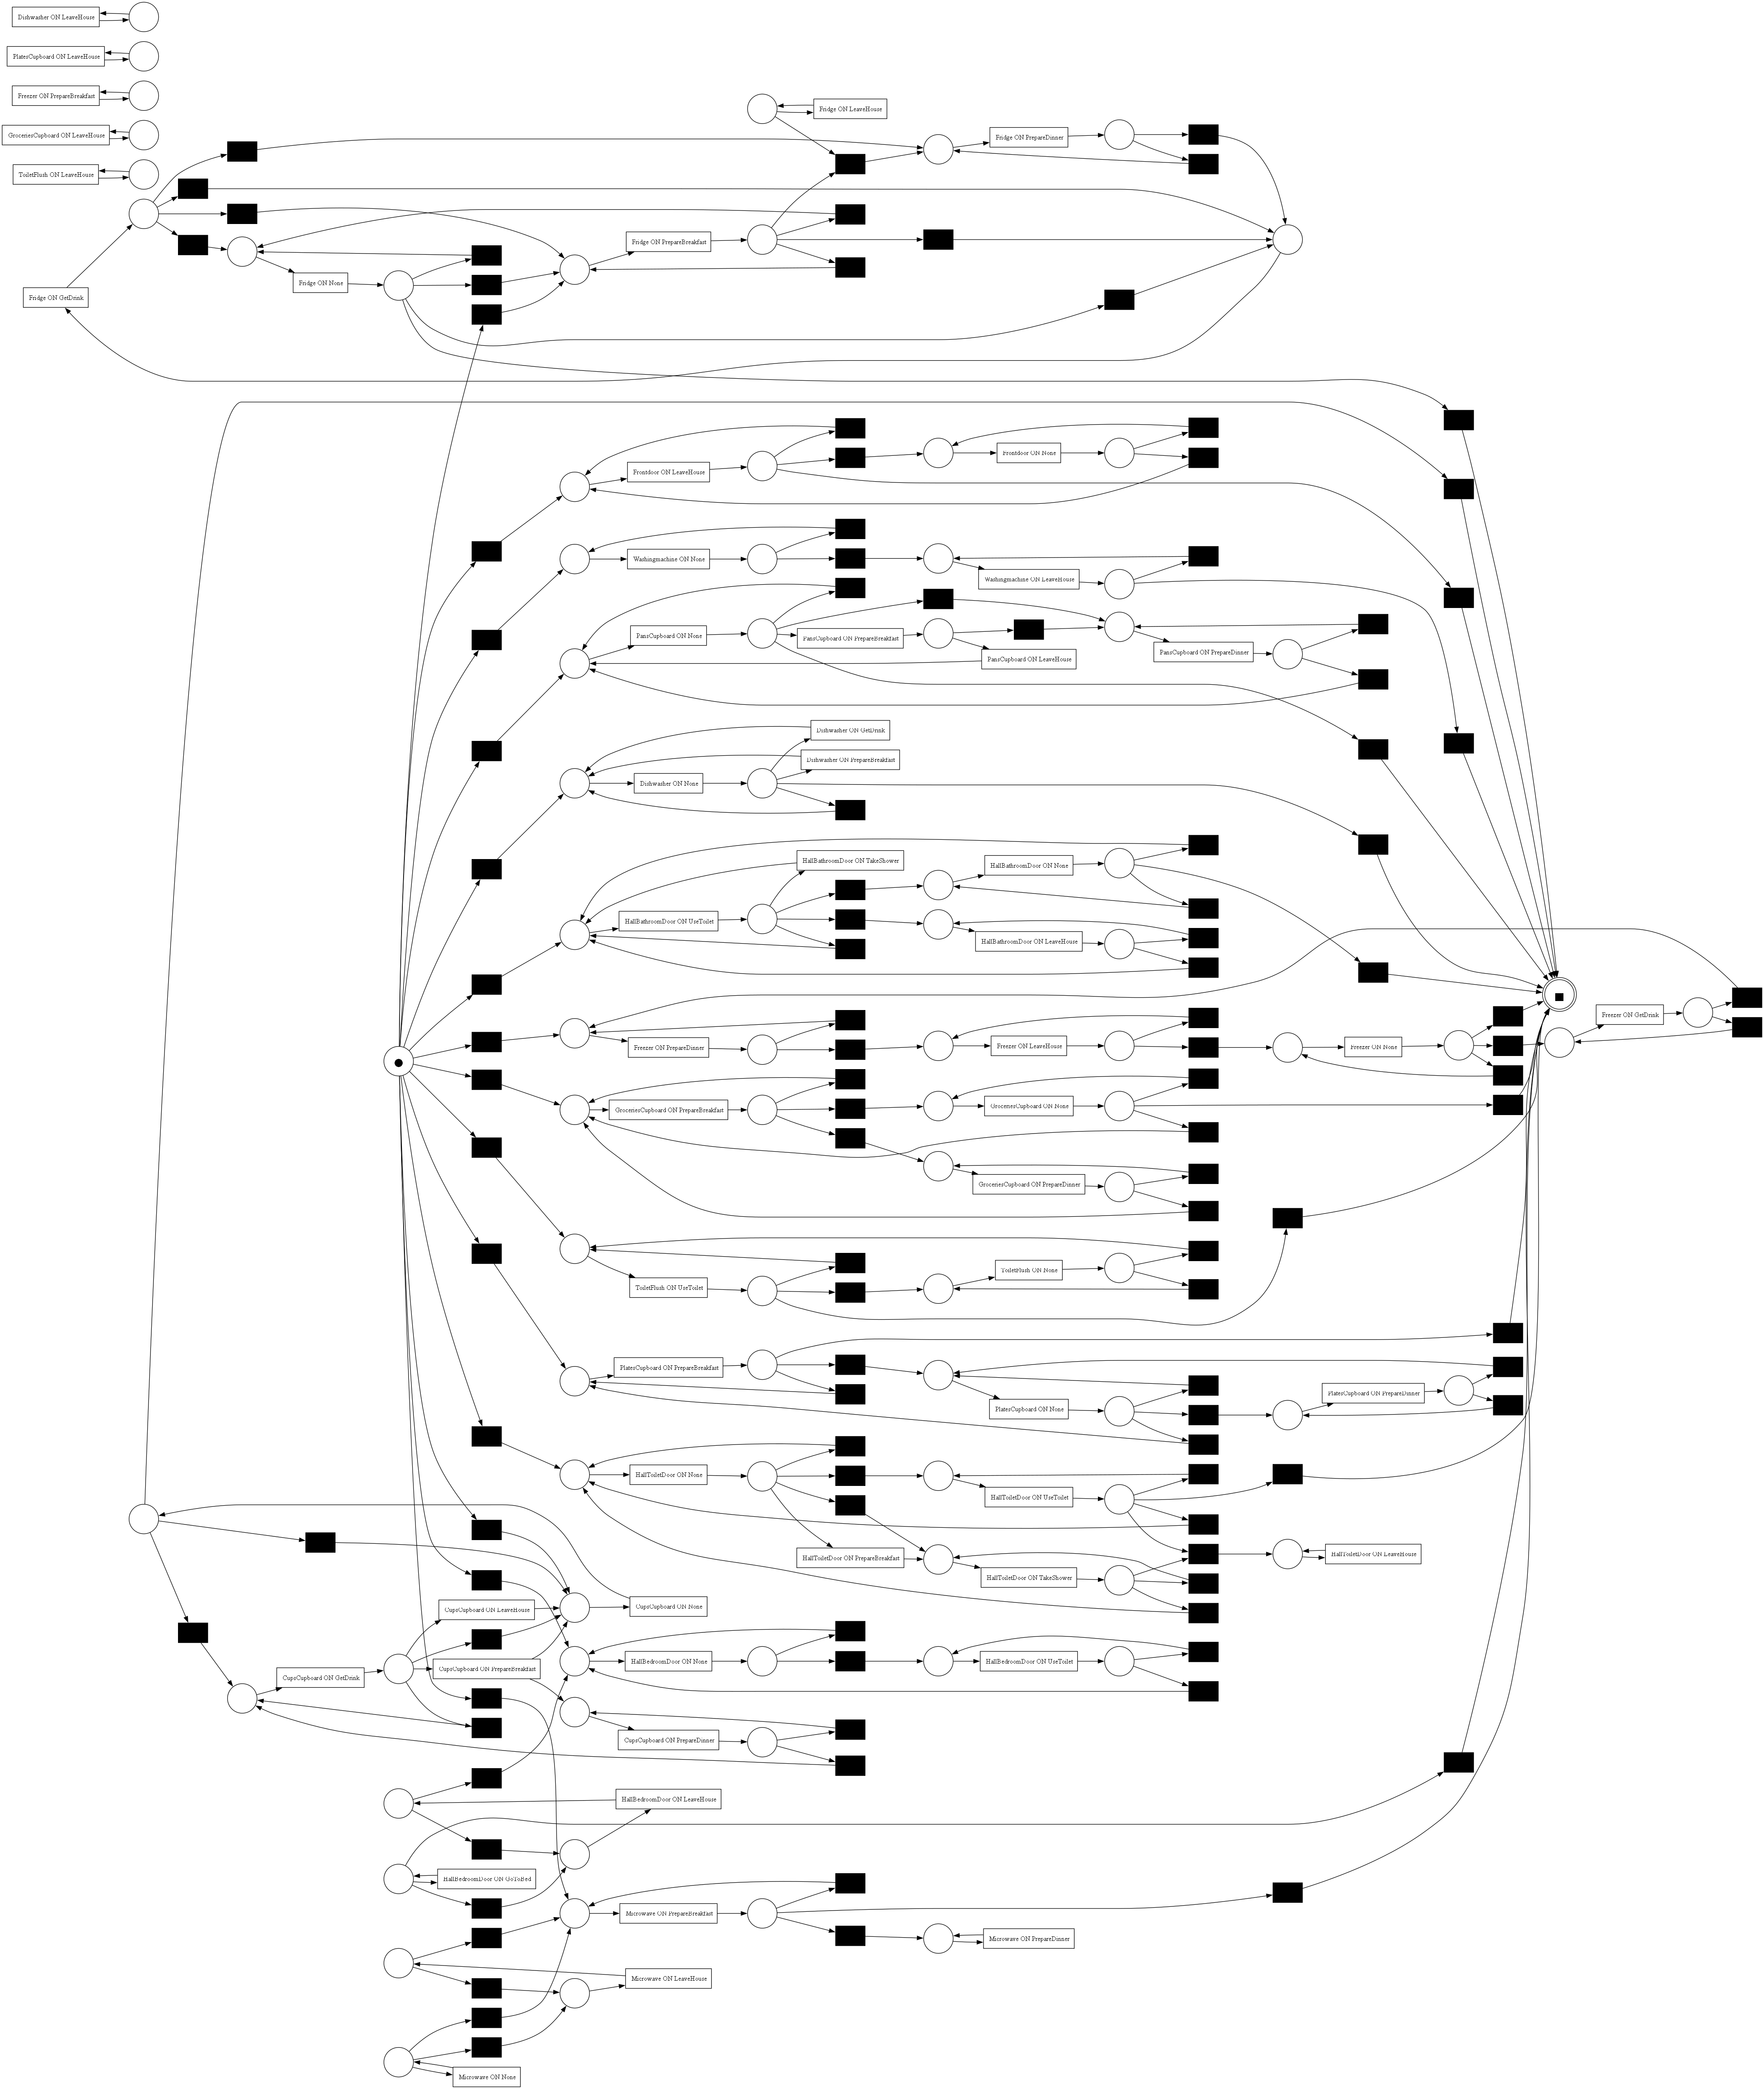
\includegraphics[width=\linewidth, height=\textheight]{images/heuristic_miner.png}
    \caption{Heuristic Miner Petri Net}
\end{figure}

\begin{figure}[H]
    \centering
    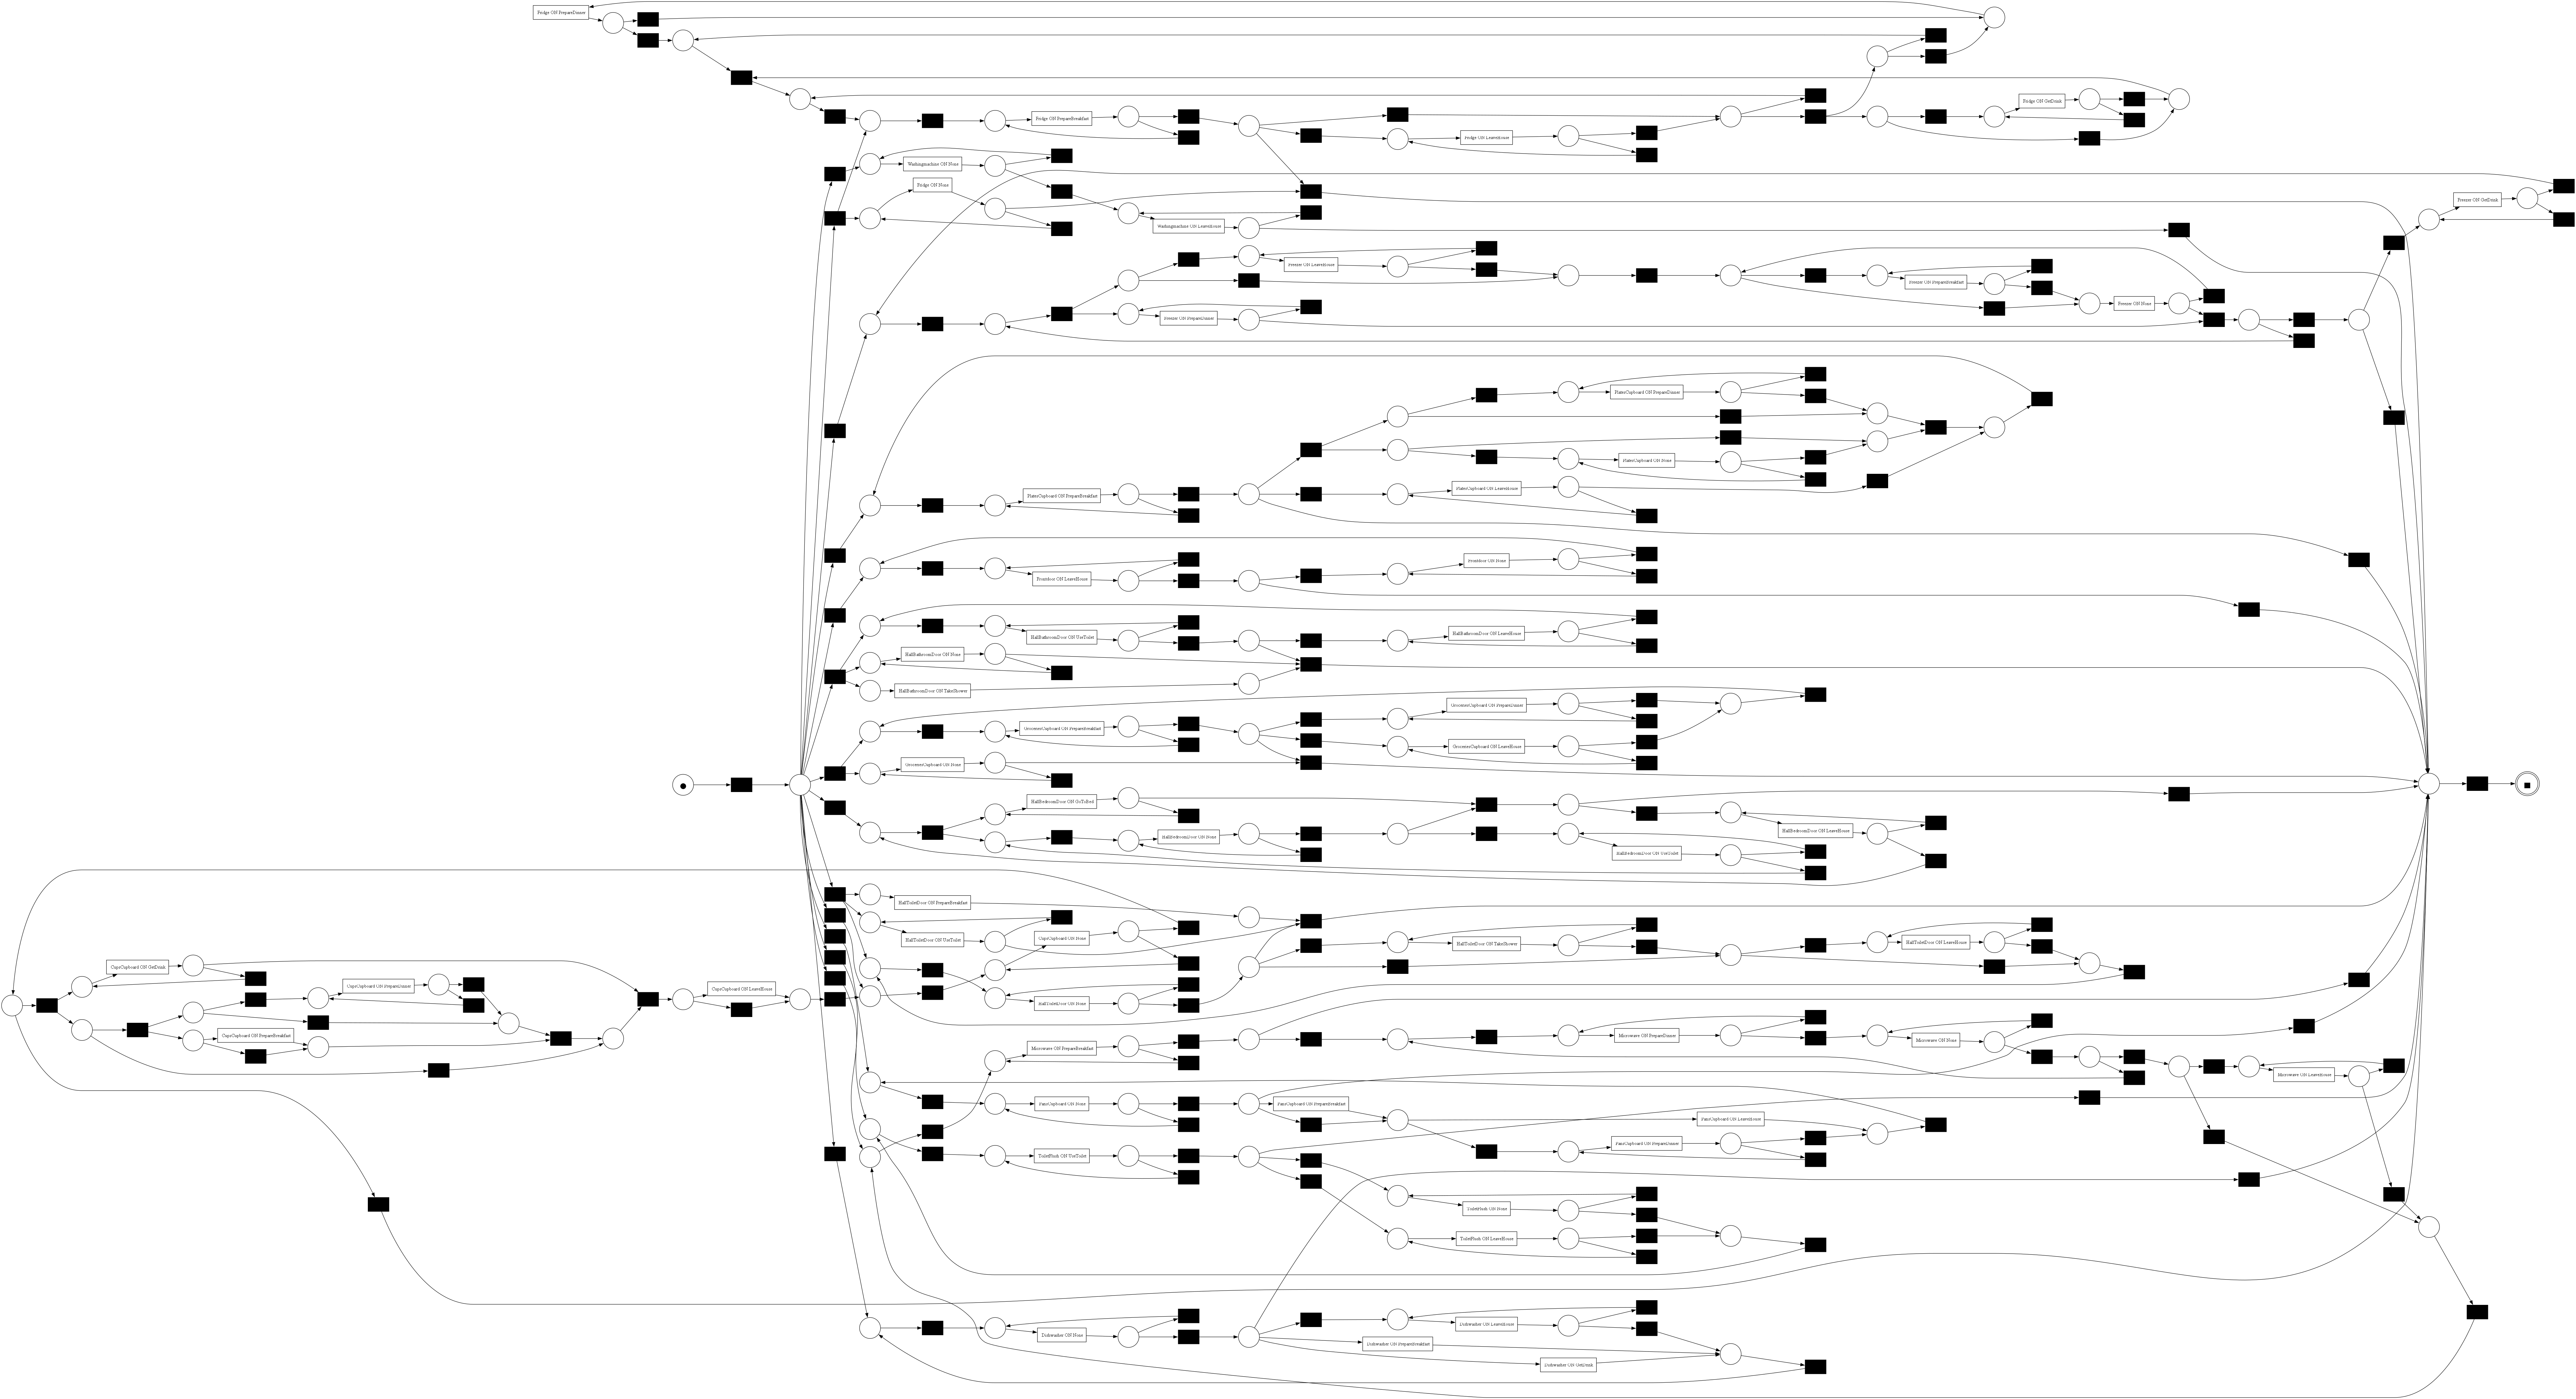
\includegraphics[width=\linewidth, height=\textheight]{images/inductive_miner.png}
    \caption{Inductive Miner Petri Net}
\end{figure}



\begin{figure}[H]
    \centering
    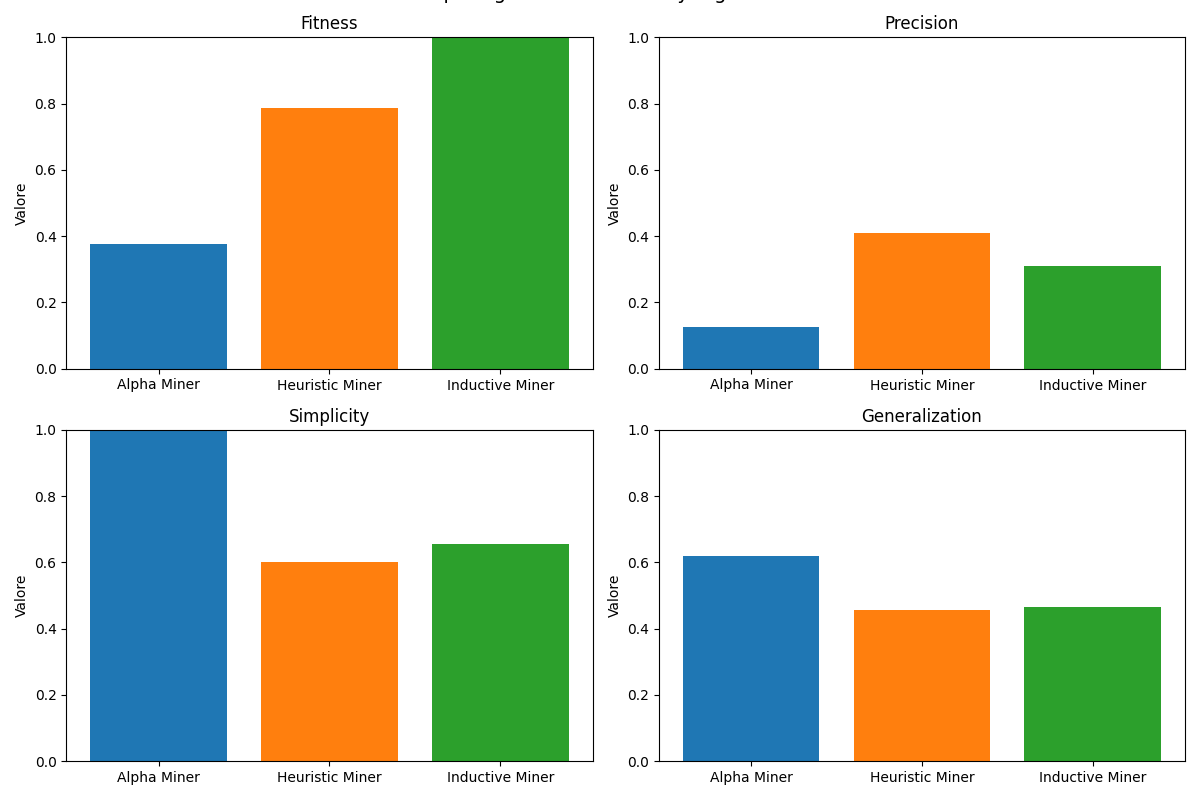
\includegraphics[scale=0.5]{images/metrics.png}
    \caption{Performance metrics of the process mining algorithms}
\end{figure}

As we can see, the Alpha Miner algorithm produces a simple PetriNet and doesn't perform very well on the other metrics
The Inductive Miner is probably the best algorithm for this dataset


\end{document}